\phantomsection
\chapter{Dependensee}
\markboth{Dependensee}{}
\label{cap5:dependensee}
% [titolo ridotto se non ci dovesse stare] 
\begin{center}
    
\includegraphics[width=.5\columnwidth]{capitoli/figure/logo_dependensee}
\end{center}

In questo capitolo verr\`{a} introdotto \textit{Dependensee}, lo strumento sviluppato per la visualizzazione di insiemi minimali di \acrfull{rfds} mediante l'implementazione della metafora visiva descritta nel paragrafo \ref{section:visual_rep_metaphore}. Tale strumento facilita la visualizzazione delle \acrfull{rfds} minimali e rappresenta diverse loro caratteristiche, facilitando l'utente nell'analisi visiva degli insiemi composti da queste.

\section{Introduzione} %\label{1sec:scopo}
Dependensee \`{e} una web application che mira a rappresentare visivamente grandi insiemi minimali di \acrfull{rfds}, per permettere all'utente che lo utilizza una rapida e semplice analisi visiva di questi insiemi. Ci\`{o} avviene attraverso ad una metafora intuitiva, descritta nel capitolo \ref{section:visual_rep_metaphore}, la quale fornisce una panoramica generale sull'insieme, esplicitando dettagli e caratteristiche delle \acrfull{rfds} che formano l'insieme. Per quanto concerne lo sviluppo, sono state utilizzate diverse tecnologie:
\begin{itemize}
    \item TypeScript,
    \item Angular,
    \item Ionic,
    \item D3.js.
\end{itemize}
TypeScript \`{e} un linguaggio di programmazione open source sviluppato da Microsoft, nato dal crescente bisogno di un linguaggio front-end per lo sviluppo di applicazioni JavaScript su larga scala. Il linguaggio nasce dalla necessit\`{a} di sicurezza e robustezza, sia da sviluppatori interni a Microsoft sia clienti. Si tratta di un super-set di JavaScript che basa le sue caratteristiche su ECMAScript 6. Estende la sintassi di JavaScript, in questo modo qualunque programma scritto in JavaScript \`{e} anche in grado di essere eseguito con TypeScript senza alcuna modifica. Inoltre, \`{e} stato progettato principalmente per lo sviluppo di applicazioni e viene successivamente ricompilato in JavaScript per poter essere interpretato in qualsiasi web browser e su qualsiasi sistema operativo.\par
Angular, evoluzione di AngularJS, \`{e} una piattaforma open source per lo sviluppo di applicazioni web. Essa \`{e} sviluppata da Google ed il linguaggio di programmazione utilizzato da Angular \`{e} TypeScript. Le applicazioni sviluppate in Angular vengono eseguite internamente dal web browser dopo essere state scaricate dal server. Il codice generato da Angular \`{e} supportato su tutti i principali web browser, da computer a mobile. Infatti, Angular \`{e} stato sviluppato con l'obiettivo di fornire uno strumento facile e veloce per lo sviluppo di applicazioni per qualunque piattaforma, inclusi smartphone e tablet.\par
Ionic \`{e} una SDK\footnote{Un \textbf{Software Development Kit (SDK)} indica un insieme di strumenti per lo sviluppo e la documentazione di software.} open source completa per lo sviluppo di app ibride, sviluppata da Drifty. Essa fornisce strumenti e servizi per lo sviluppo di applicazioni desktop, mobile e Progressive Web Apps, basate sulle pratiche e tecnologie moderne di sviluppo web, utilizzando tecnologie come CSS, HTML5 e SASS. In particolare, possono essere sviluppate applicazioni mobile con le suddette tecnologie web ed \`{e} possibile, successivamente, distribuirle tramite Cordova o Capacitor sui vari App Store nativi.\par
D3.js \`{e} una libreria sviluppata in JavaScript per creare visualizzazioni dinamiche ed interattive partendo da dati organizzati, visibili attraverso un comune browser. Per fare ci\`{o} si serve largamente degli standard web: SVG, HTML5 e CSS. Diversamente da molte altre librerie, essa permette un ottimo controllo e resa visiva sul risultato finale. D3.js, incorporata in una pagina web HTML, utilizza funzioni JavaScript prefatte per selezionare elementi del DOM, creare elementi SVG, aggiungergli uno stile grafico, oppure transizioni, effetti di movimento e/o tooltip. Questi oggetti possono essere personalizzati utilizzando il CSS. In questo modo grandi collezioni di dati possono essere facilmente convertiti in oggetti SVG usando semplici funzioni della libreria e cos\`{i} generare ricche rappresentazioni grafiche di numeri, testi, mappe e diagrammi. I dati utilizzati possono essere in diversi formati, i pi\`{u} comuni sono JSON e CSV, ma, se necessario, si possono scrivere funzioni per leggere dati in altri formati.

\section{Funzionamento}

L'utilizzo di Dependensee \`{e} molto semplice. Il deploy dell'applicazione pu\`{o} essere effettuato sia su server che in locale. Per effettuare il deploy in locale \`{e} necessario, come prerequisiti, avere Node.js, npm ed Ionic 4 sulla propria macchina. Successivamente, basta aprire la directory tramite bash e digitare il comando \texttt{ionic serve}, cos\`{i} da avviare un server in locale su tutte le interfacce di rete. Fatto ci\`{o}, baster\`{a} dirigersi all'indirizzo corrispondente al server avviato, in genere \texttt{http://localhost:8100}, per iniziare ad utilizzare Dependensee. Una volta aperto l'indirizzo nel browser, si presenter\`{a} un'interfaccia semplice ed immediata, come mostrato in Figura \ref{fig:dependensee_main_screen}, composta da:
\begin{itemize}
    \item un input per selezione il dataset da analizzare in formato .txt,
    \item un input per indicare la threshold massima,
    \item un bottone per avviare l'analisi e generare il grafico relativo al dataset,
    \item una finestra nascosta di default che \`{e} possibile mostrare per leggere i messaggi di log generati da Dependensee.
\end{itemize}
% -- Main Screen
\begin{figure}[ht]
    \centering
    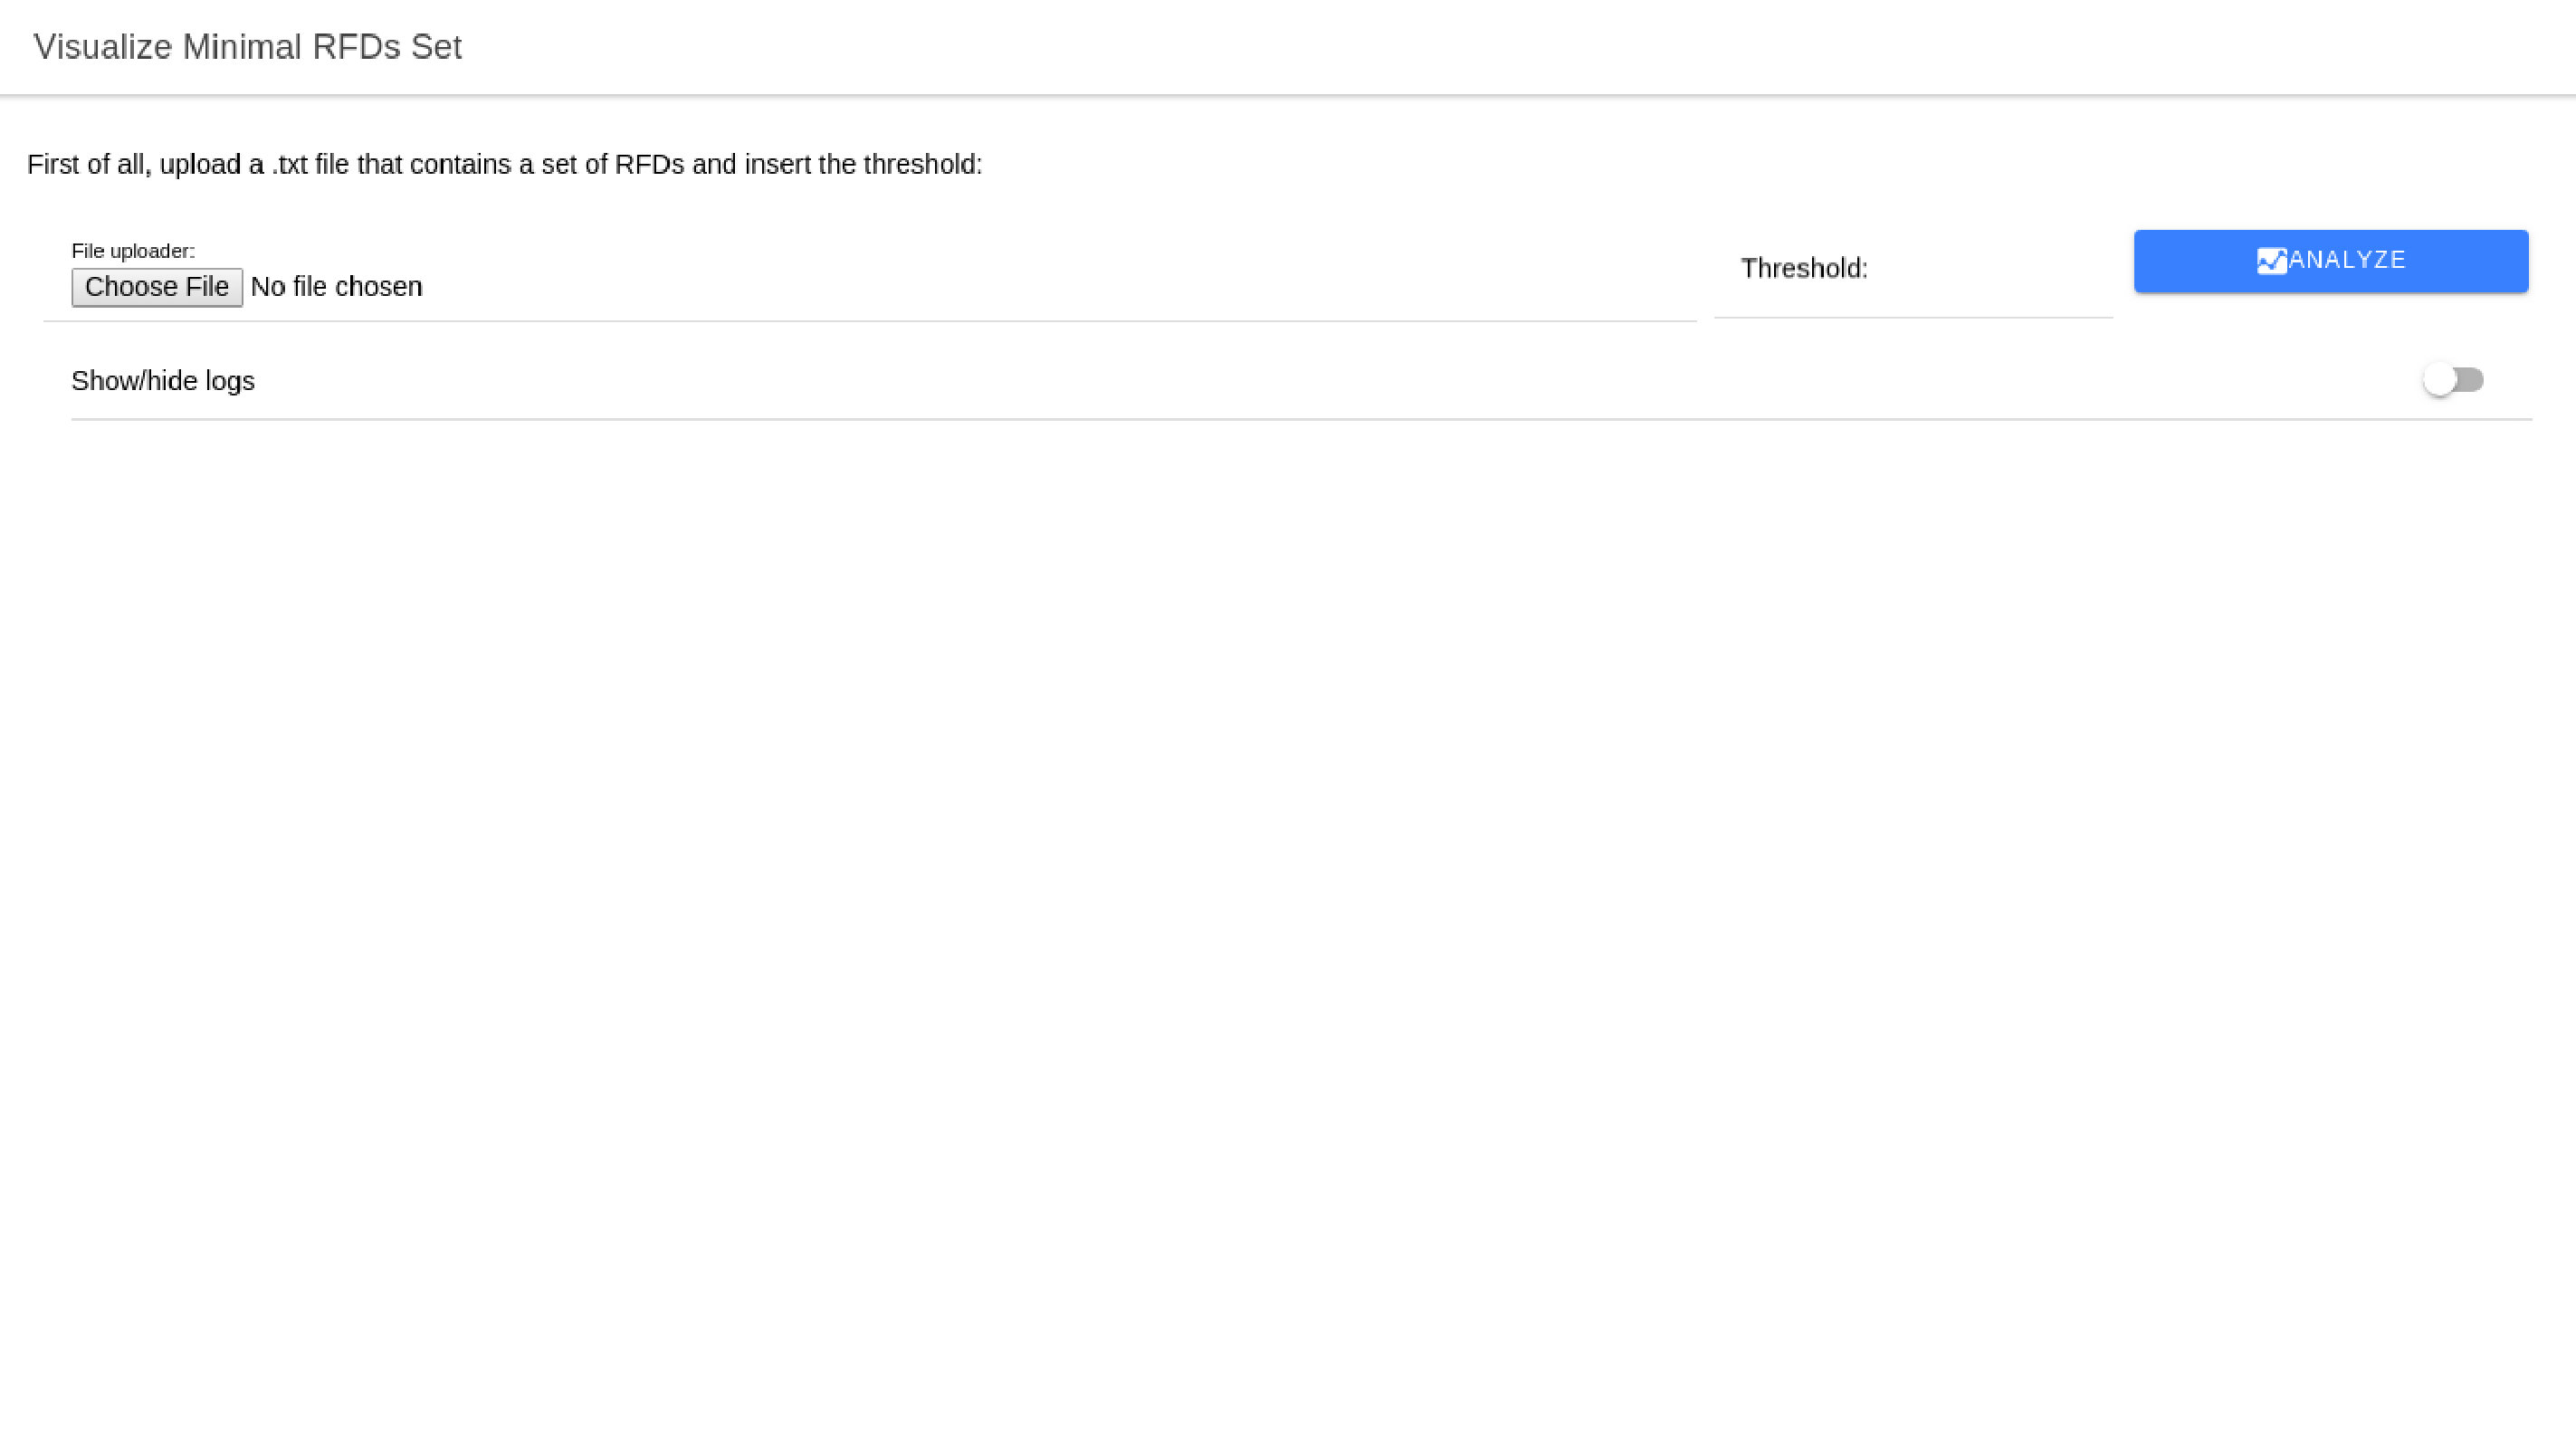
\includegraphics[width=\linewidth]{capitoli/figure/dependensee_main_screen}
    \caption{Interfaccia di Dependensee.}
    \label{fig:dependensee_main_screen}
\end{figure}
% -- End Main Screen
Quindi, bisogna selezionare il dataset da analizzare in formato .txt, con la seguente struttura:
\begin{verbatim}
    B@4.0->F@4.0
    D@4.0->F@4.0
    C@4.0->F@4.0
    E@4.0->F@4.0
    G@4.0->F@4.0
    A@4.0->F@4.0
    A@2.0,B@0.0,C@0.0,D@4.0,E@2.0,F@2.0->G@2.0
    A@0.0,B@0.0,C@0.0,D@4.0,E@2.0,F@2.0->G@0.0
\end{verbatim}
dove le stringhe che precedono il simbolo \texttt{@} indicano gli attributi, i valori che vengono scritti dopo il simbolo \texttt{@} indicano le threshold relative agli attrubuti ed i simboli \texttt{->} dividono il lato sinistro della \acrshort{rfd} dal lato destro. Successivamente, bisogna inserire il valore massimo delle threshold e cliccare sul bottone per avviare l'analisi. Se i due campi di input non sono stati violati, allora Dependensee proceder\`{a} con l'analisi e visualizzer\`{a} un grafico relativo al dataset inserito, come mostrato in Figura \ref{fig:dependensee_dataset_analyzed}, altrimenti mostrer\`{a} un messaggio d'errore relativo al campo di input da modificare.
% -- Dataset Analyzed
\begin{figure}[ht]
    \centering
    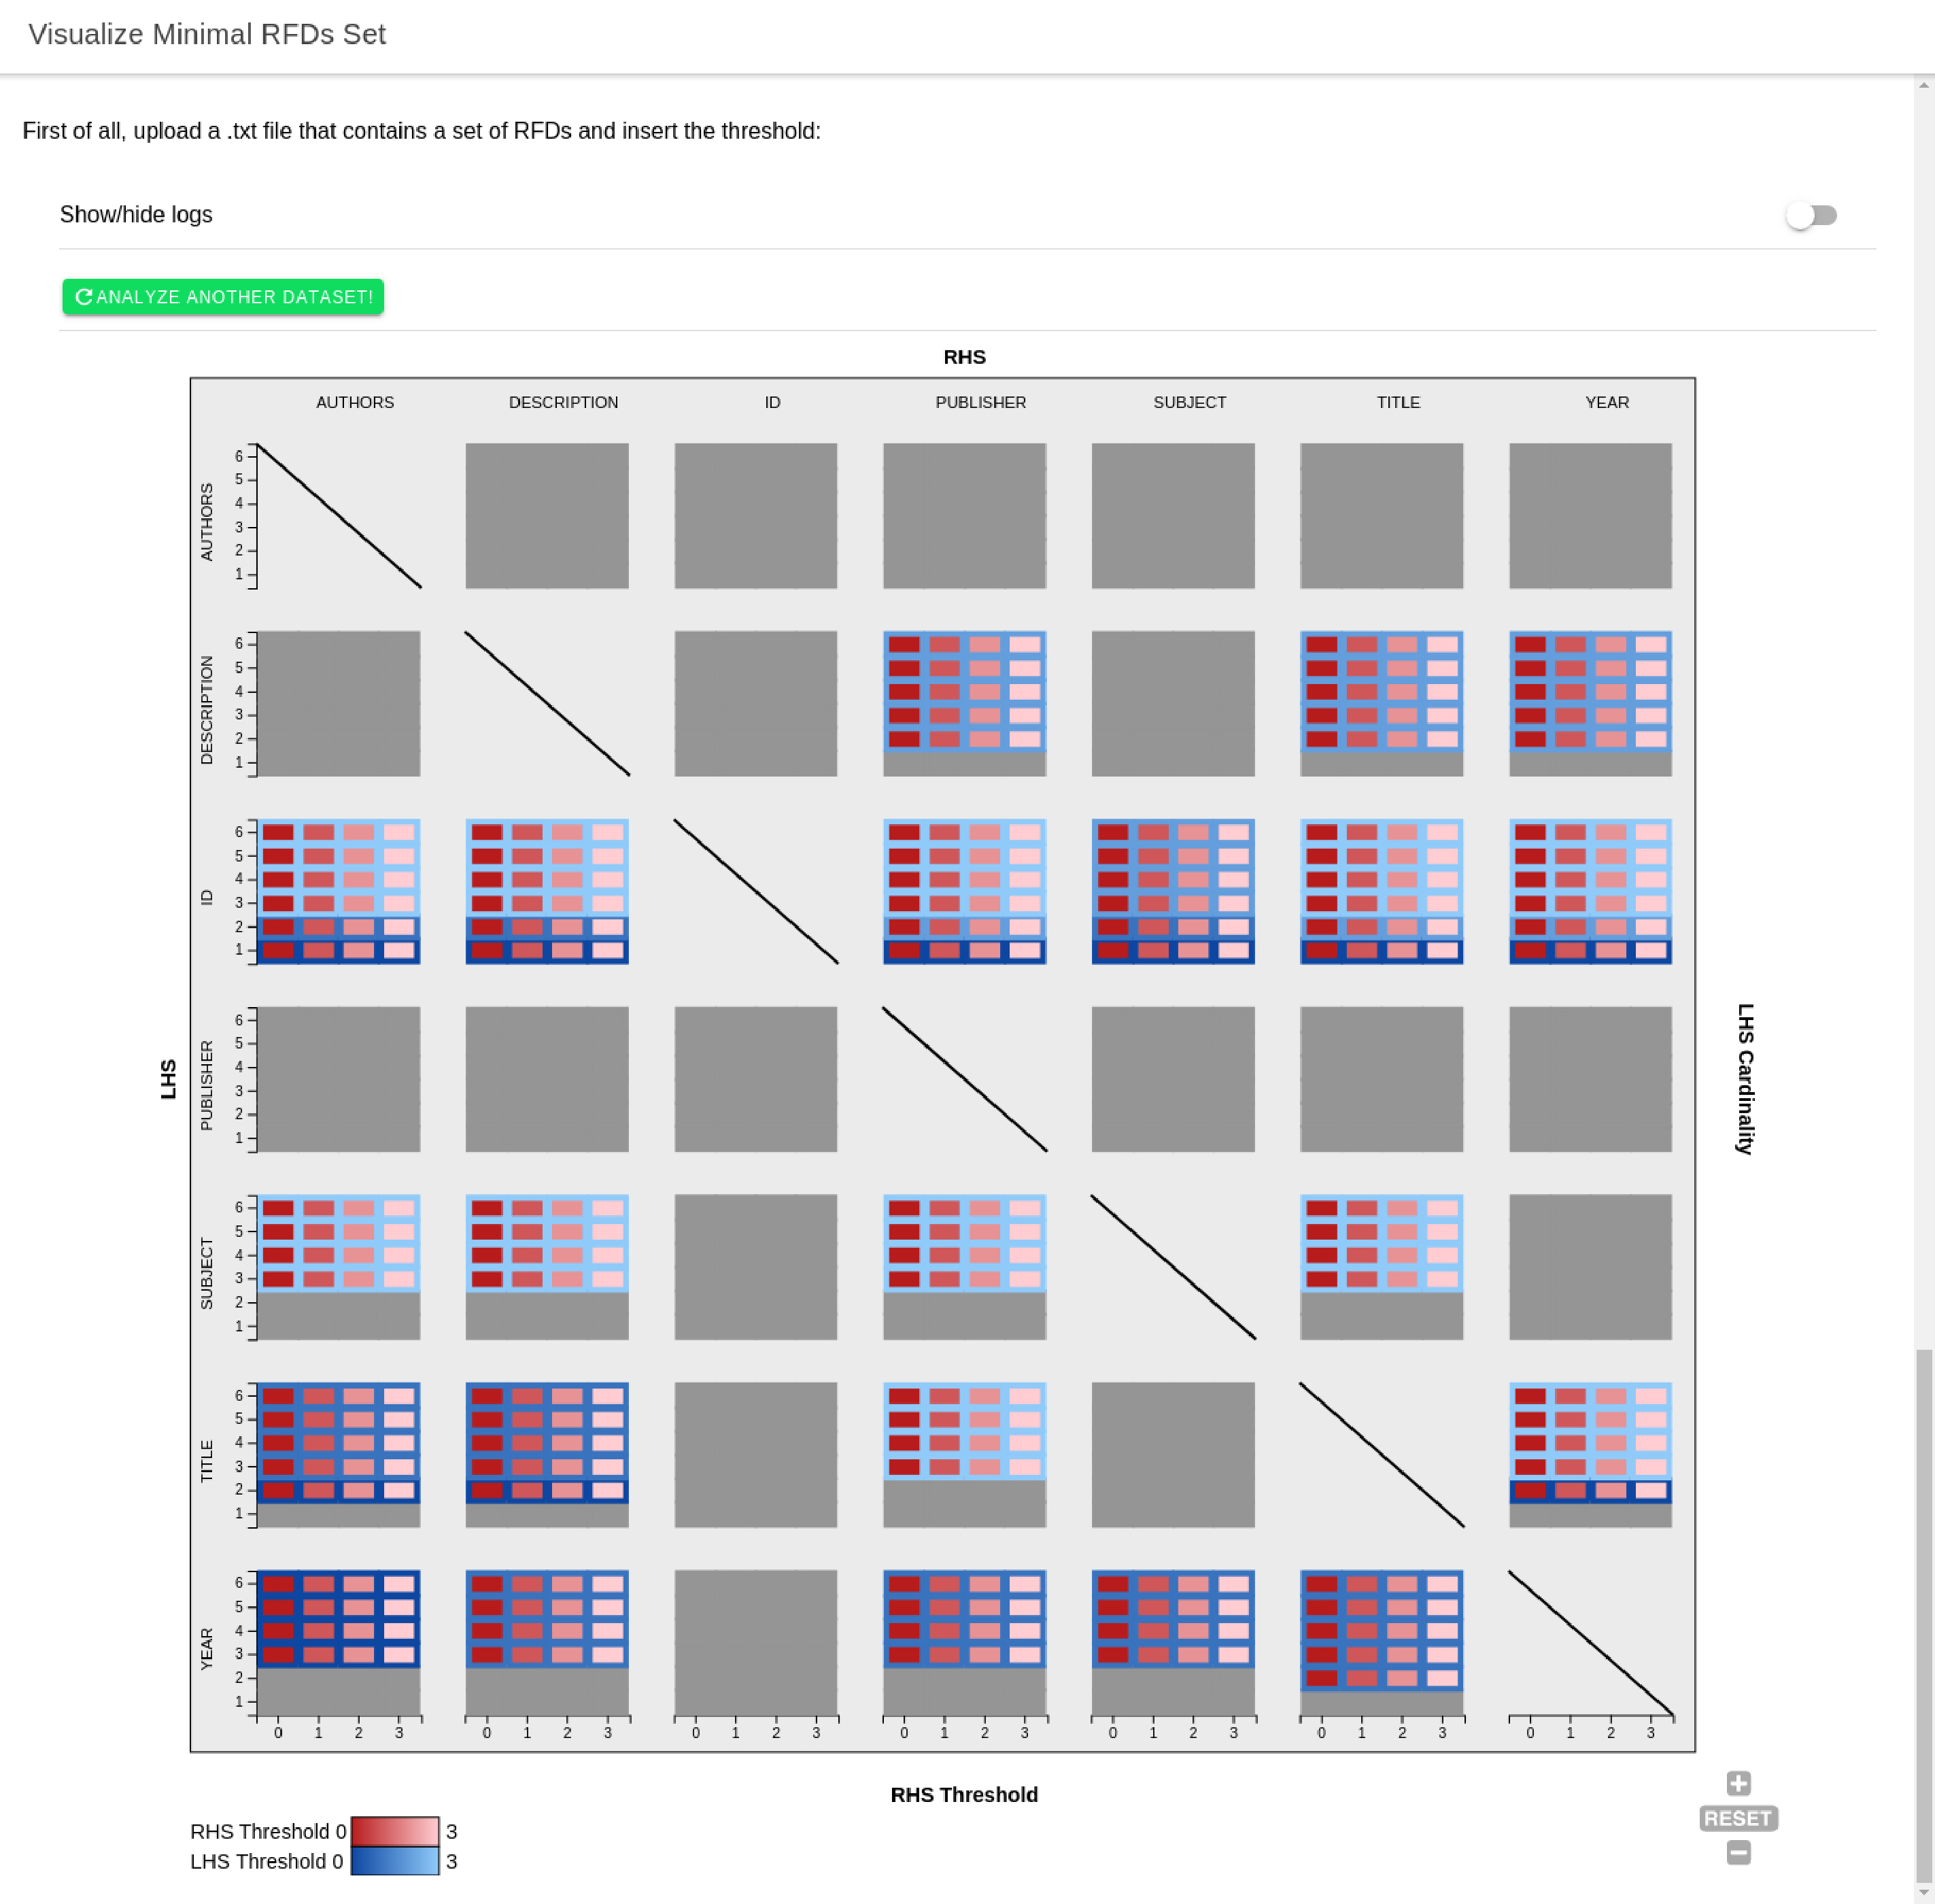
\includegraphics[width=\linewidth]{capitoli/figure/dependensee_analyzed_screen}
    \caption{Grafico generato da Dependensee relativo al dataset inserito in input.}
    \label{fig:dependensee_dataset_analyzed}
\end{figure}
% -- End Dataset Analyzed
Una volta analizzato il dataset sar\`{a} possibile effettuare operazioni di zoom-in/out per visualizzare meglio il grafico e singole porzioni di esso, oppure sar\`{a} possibile analizzare un altro dataset cliccando sul bottone in alto.